\documentclass[11pt]{beamer}
\usetheme{Warsaw}
\usepackage[utf8]{inputenc}
\usepackage{amsmath}
\usepackage{amsfonts}
\usepackage{amssymb}
\usepackage{graphicx}
%\author{}
%\title{}
%\setbeamercovered{transparent} 
%\setbeamertemplate{navigation symbols}{} 
%\logo{} 
%\institute{} 
%\date{} 
%\subject{} 
\begin{document}

%\begin{frame}
%\titlepage
%\end{frame}

%\begin{frame}
%\tableofcontents
%\end{frame}

\begin{frame}{Versuchsbeschreibung}
\section{Auf- und Entladung eines Kondensators, Teilversuch 4.2}
\subsection{Versuchsbeschreibung}
\subsubsection*{Aufladung}
\begin{itemize}
\item Strom- bzw. Spannungsverlauf messen
\item Zeitkonstante bestimmen
\[\tau = R \cdot C \]
\item Aufladung:
\begin{align*}
U_0-U_R(t)-U_C(t)=0 \rightarrow U_0-U_C(t)=I(t) \cdot R
\end{align*}
\begin{align*}
U_C(t)=U_0 \cdot (1-e^{-\frac{t}{R \cdot C}}) \hspace{2cm} I(t)=I_0 \cdot e^{-\frac{t}{R \cdot C}}
\end{align*}
\subsubsection*{Entladung}
\item Entladung:
\begin{align*}
R \cdot I(t) + U_C(t) = 0
\end{align*}
\begin{align*}
U_C(t)=U_0 \cdot e^{-\frac{t}{\tau}} \hspace{2cm} I(t)=-\frac{U_0}{R} \cdot e^{-\frac{t}{\tau}}
\end{align*}
\end{itemize}
\end{frame}
\begin{frame}{Versuchsaufbau}
\subsection{Versuchsaufbau und Durchführung}
\begin{figure}[hbtp]
\centering
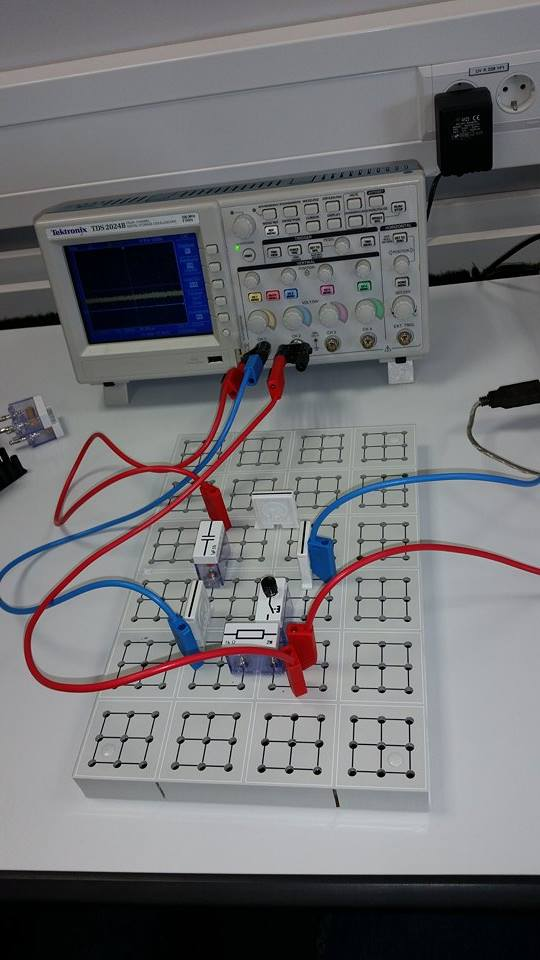
\includegraphics[scale=0.19]{12834525_1207198235971903_753892727_n.jpg}
\caption{Versuchsaufbau}
\end{figure}
\end{frame}
\begin{frame}{Versuchsauswertung}
\begin{itemize}
\subsection{Versuchsauswertung}
\item Offsests korrigiert
\item Aus abgelesenen Werten $\tau$ berechnen:
\begin{align*}
\frac{U_1}{U_2}=e^{-\frac{t_1-t_2}{\tau}}
\end{align*}
\begin{align*}
\tau=\frac{\Delta t}{\ln{\frac{U_1}{U_2}}} \hspace{1cm}
\sigma_{\tau}=\sqrt{(\frac{\sigma_{\Delta t}}{\ln{\frac{U_1}{U_2}}})^2+(\frac{\Delta t}{U_1} \cdot \sigma_{U_1})^2+(-\frac{\Delta t}{U_2} \cdot \sigma_{U_2})^2}
\end{align*}
\item Aus $\tau$ $C$ bestimmen
\item sys. Fehler auf $C$ ergibt sich aus:
\begin{align*}
\frac{\sigma_{C,sys}^R}{C}=\frac{\sigma_{R,sys}}{R}
\end{align*}
\end{itemize}
\end{frame}
\begin{frame}{Rohdaten}
\begin{itemize}
\subsubsection{Rohdaten}
\item Werte für $U$ und $I$ im Abstand von $1ms$ notiert
\item Ablesefehler notiert
\begin{table}[H]\centering
\caption{Oszilloskop}
\begin{tabular}{c|c}
$I_1$& $I_2$\\ \hline
$0,72A$& $1,88A$\\ 
$0,8A$& $2,24A$ \\
$0,76A$& $2,12A$ \\
$0,72A$& $1,92A$ \\
\\
$U_1$& $U_2$ \\ \hline
$0,84V$& $2,48V$ \\
$0,84V$& $2,44V$ \\
$0,80V$& $2,40V$ \\
$0,89V$& $2,44V$ \\
\end{tabular} 
\end{table}
\end{itemize}
\end{frame}
\begin{frame}{Analyse/Transformation der Rohdaten}
\begin{itemize}
\subsubsection{Analyse/Transformation der Rohdaten}
\item $\tau$ und $\sigma_{\tau}$ berechnet
\item $C$ und $\sigma_C$ berechnet:
\begin{align*}
C=\frac{\tau}{R} \hspace{2cm} \sigma_C=\sqrt{(\frac{\sigma_{\tau}}{R})^2+(-\frac{\tau}{R^2}\cdot \sigma_R)^2}
\end{align*}
\item Der systematische Fehler aus Widerstandsmessung berechnet
\item Einzelergebnisse mit Gesammtfehlern gegen Mittelwert geplottet
\end{itemize}
\end{frame}
\begin{frame}{Ergebnis}
\begin{figure}[hbtp]
\centering
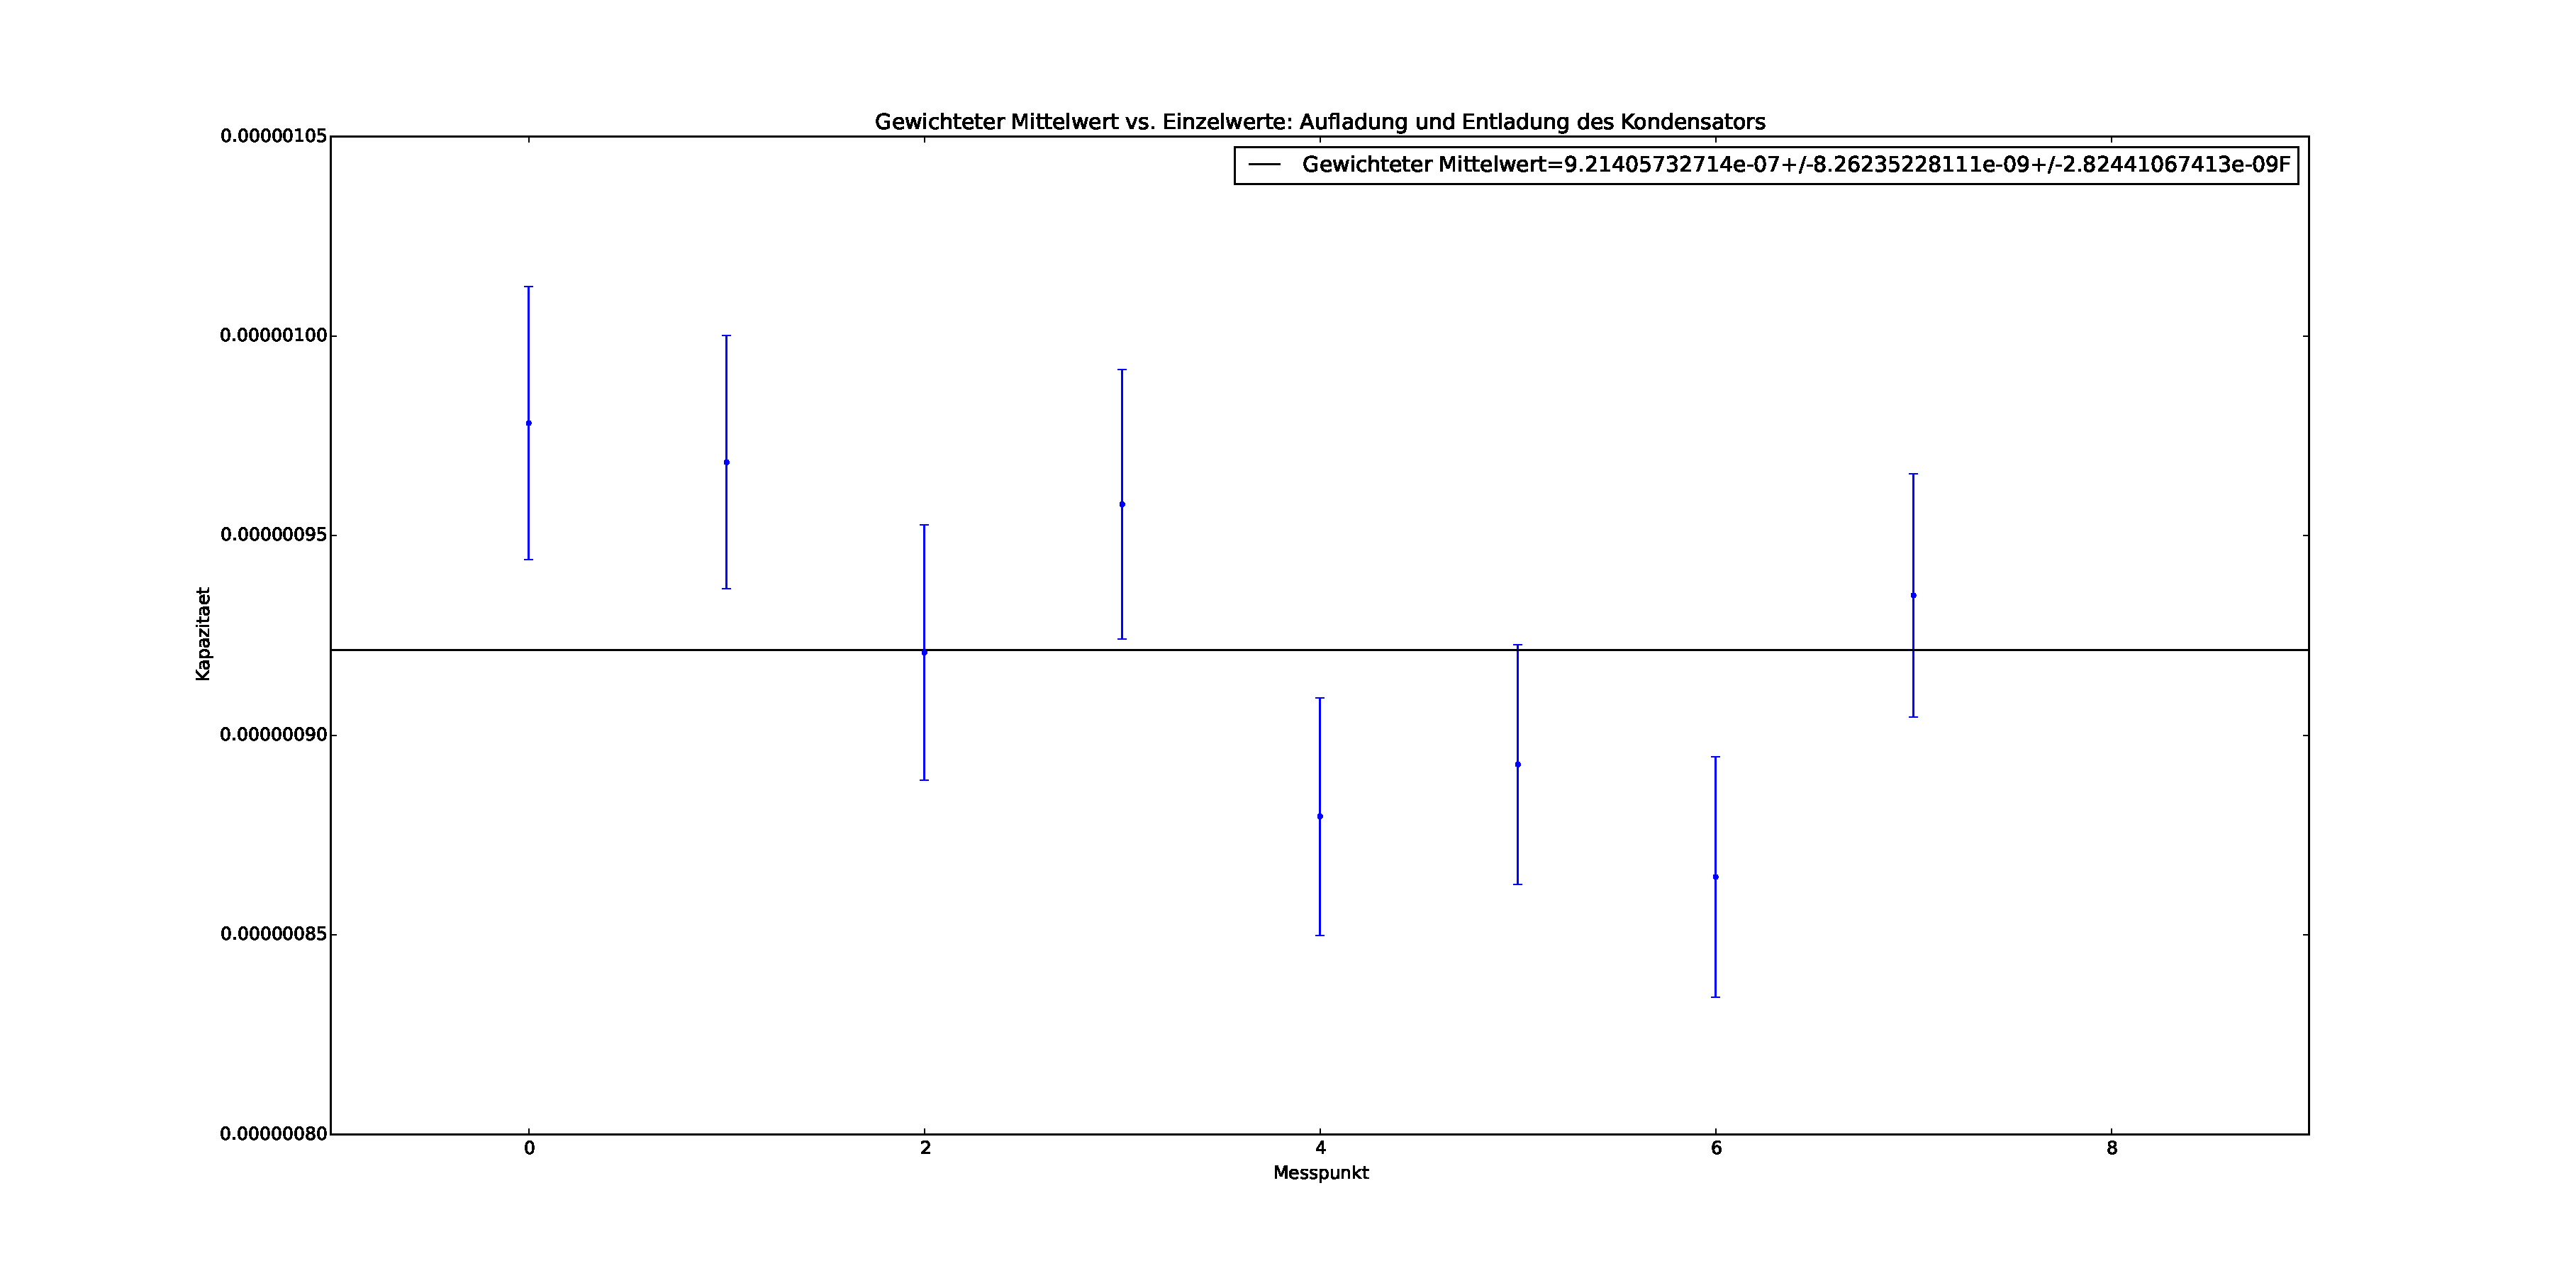
\includegraphics[scale=0.2]{auf-entladung.eps}
\caption{Ergebnisse vs. Mittelwert}
\end{figure}
\end{frame}
\begin{frame}{Fazit}
\subsubsection{Fazit}
\begin{itemize}
\item Drei Werte im Bereich $1\sigma$ vom Mittelwert
\item Alle Werte im Bereich $2\sigma$ vom Mittelwert
\item Abweichung zum Literaturwert durch nicht berücksichtigte sys. Fehler: z.B. Widerstand der Kabel
\end{itemize}
\end{frame}

\end{document}